{\renewcommand{\arraystretch}{1.4}
\begin{landscape}
\chapter{Actieplan}
	\vspace{-3cm}
	
	\begin{table}[htbp]
		\centering
		\begin{tabular}{|l|p{0.5\linewidth}|l|l|l|}
			\hline
			\multicolumn{1}{|c|}{\textit{\textbf{Milestones}}}&
			\multicolumn{1}{|c|}{\textit{\textbf{Taak}}}&
			\multicolumn{1}{|c|}{\textit{\textbf{Start datum}}} & \multicolumn{1}{c|}{\textit{\textbf{Eind datum}}} &
			\multicolumn{1}{c|}{\textit{\textbf{Duur}}} \tabularnewline \hline
			Milestone 1 & Defining Architecture/Data Model & 6/02/2017 & 10/02/2017 & 4\tabularnewline \hline
			Milestone 2 & Test scripts for uploading avatars/cover photos for Faceboo/Twitter & 13/02/2017 & 17/02/2017 & 4\tabularnewline \hline
			Milestone 3 & Theme creation (Name, Type, Images, Link color) & 20/02/2017 & 24/02/2017 & 4\tabularnewline \hline
			Milestone 4 & Selecting multiple themes for profiles & 27/02/2017 & 03/03/2017 & 4\tabularnewline \hline
			Milestone 5 & Applying thems (cron jobs/scheduled) & 06/03/17 & 10/03/17 & 4\tabularnewline \hline
			Milestone 6 & Update profile name/link/bio (Twitter) & 13/03/17 & 17/03/17 & 4\tabularnewline \hline
			Milestone 7 & Annotations & 20/03/17 & 7/04/17 & 12\tabularnewline \hline
			Milestone 8 & Annotations with KPI & 20/03/17 & 7/04/17 & 12\tabularnewline \hline
			Milestone 9 & Define welcome messages for profile (Optional) & 10/04/17 & 21/04/17 & 8\tabularnewline \hline
			Milestone 10 & Define persistent menu for Facebook (Optional) & / & / & /\tabularnewline \hline
			Milestone 11 & Integration in Crisis Plans & 24/04/17 & 28/04/17 & 4\tabularnewline \hline
			Milestone 12 & Theme preview (Optional) & / & / & /\tabularnewline \hline
			Milestone 13 & Asset Gallery in Theme Builder (Optional) & / & / & /\tabularnewline \hline
			Milestone 14 & Depolyment & 1/05/17 & 5/05/17 & 4\tabularnewline \hline
			Milestone 15 & Testing & 8/05/17 & 12/05/17 & 4\tabularnewline \hline
			 
		\end{tabular}
		\caption{Milestones Profile Manager}
		\label{tabelActieplan}   
	\end{table}
	
	
	
	\newpage
	
	\begin{figure}[H]
		\centering
		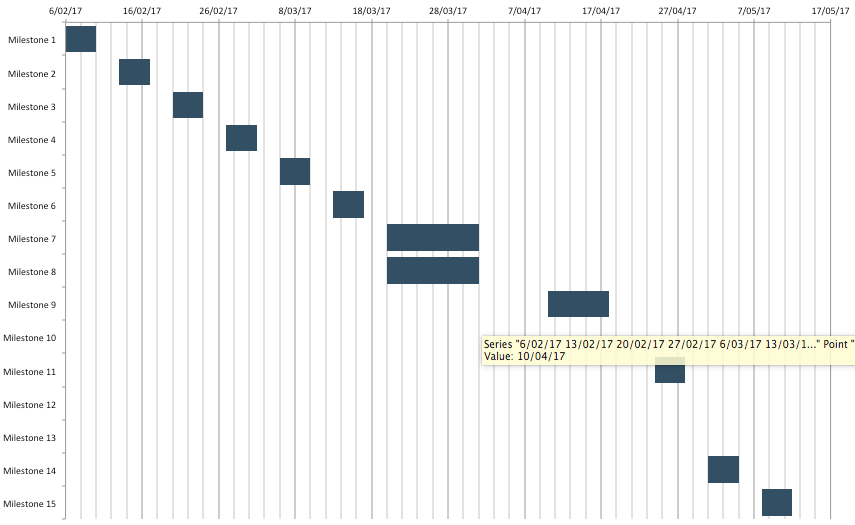
\includegraphics[width=1.5\textwidth]{Figuren/GanttChartDark.png}
		\caption{Gantt chart - Profile Manager} %\cite{Pouladzadeh}
		%\label{fig:Actieplan}
	\end{figure}
\end{landscape}